\documentclass[12pt]{article}

\usepackage[utf8x]{inputenc} % Включаем поддержку UTF8  
\usepackage[russian]{babel}  % Включаем пакет для поддержки русского языка  
\usepackage{hyperref}        % Для гиперссылок

% Математика
\usepackage{amsmath,amsfonts,amssymb,amsthm,mathtools} % AMS
\usepackage{icomma}
\usepackage{mathrsfs}

\usepackage{xcolor}

% Прога
\usepackage{etoolbox}
\usepackage{listings}

\definecolor{codegreen}{rgb}{0,0.6,0}
\definecolor{codegray}{rgb}{0.5,0.5,0.5}
\definecolor{codepurple}{rgb}{0.58,0,0.82}
\definecolor{backcolour}{rgb}{0.95,0.95,0.92}

\lstdefinestyle{mystyle}{
	backgroundcolor=\color{backcolour},   
	commentstyle=\color{codegreen},
	keywordstyle=\color{magenta},
	numberstyle=\tiny\color{codegray},
	stringstyle=\color{codepurple},
	basicstyle=\ttfamily\footnotesize,
	breakatwhitespace=false,         
	breaklines=true,                 
	captionpos=b,                    
	keepspaces=true,                 
	numbers=left,                    
	numbersep=5pt,                  
	showspaces=false,                
	showstringspaces=false,
	showtabs=false,                  
	tabsize=2
}

\lstset{style=mystyle}

% Цвета
\usepackage{xcolor}

% Картинки
\usepackage{graphicx}
\graphicspath{ {./images/} }

\usepackage{tikzsymbols}

% Работа с таблицами
\usepackage{array,tabularx,tabulary,booktabs} % Дополнительная работа с таблицами
\usepackage{longtable}  % Длинные таблицы
\usepackage{multirow} % Слияние строк в таблице

% Нумерованные списки
\usepackage[shortlabels]{enumitem} % Разные лейблы

% Текст
\usepackage[normalem]{ulem}  % для зачеркивания текста

\newtheorem{property}{Свойство}
\newtheorem{consequence}{Следствие}[property]

\DeclarePairedDelimiter\abs{\lvert}{\rvert}%
\DeclarePairedDelimiter\norm{\lVert}{\rVert}%

% Swap the definition of \abs* and \norm*, so that \abs
% and \norm resizes the size of the brackets, and the 
% starred version does not.
\makeatletter
\let\oldabs\abs
\def\abs{\@ifstar{\oldabs}{\oldabs*}}
%
\let\oldnorm\norm
\def\norm{\@ifstar{\oldnorm}{\oldnorm*}}
\makeatother

\begin{document}
	
	\thispagestyle{empty}
	\begin{center}
		\textbf{ПРАВИТЕЛЬСТВО РОССИЙСКОЙ ФЕДЕРАЦИИ}
		
		\vspace{5ex}
		
		\textbf{Федеральное государственное автономное образовательное учреждение \\ высшего образования \\ <<Национальный исследовательский университет \\ <<Высшая школа экономики>>}
	\end{center}
	\vspace{5ex}
	
	\begin{center}
		Московский институт электроники и математики им. А.Н. Тихонова  
		
		\vspace{5ex}
		
		Департамент прикладной математики
		
		\vspace{10ex}
		\textbf{Отчёт \\ по лабораторной работе №4 \\ по курсу <<Алгоритмизация и программирование>> \\ Задание № 13}
		\vspace{7ex}
		
	\end{center}
	
	\begin{center} 
		\begin{tabular}{| p{0.3\linewidth}| p{0.3\linewidth}| p{0.3\linewidth}|}
			\hline	
			ФИО студента & Номер группы & Дата \\  \hline
			& & \\  
			Кейер Александр \newline Петрович & БПМ-231 & 21.11.2023\\  
			& & \\  \hline		
		\end{tabular}
	\end{center}
	
	\begin{center}
		\vspace{3ex}
		
		\vfill
		
		\normalsize
		
		\textbf{Москва, 2023}
	\end{center}
	
	\newpage
	
	%---------------------------------------------------------------------------------
	
	\section*{Задание (вариант № 13)}
	
 	Числовой массив B (тип массива указан в формулировке второго задания) содержит k
    элементов. Элементы массива и пороговые значения X, Y вводятся с клавиатуры. Написать
 	подпрограммы создания массива и вывода его на экран. В первом задании требуется написать
 	функцию нахождения соответствующего варианту максимального/минимального значения, а
 	во втором – среднего арифметического указанных в условии элементов («между» понимать
 	строго – не включая найденные позиции).
 	Оба задания реализовать в одной программе.
 	\vspace{5pt}
	\newline
	\textbf{№1} $max(b_1,\ldots,b_k), X \leq b_i \leq Y$ \newline
	\textbf{№2} Среднее арифметическое элементов, расположенных до первого минимального элемента среди нечётных. Массив целочисленный.
	
	\newpage
	
	\section*{Решение}
	
	\begin{lstlisting}[language=C]
	#include <stdio.h> // Input/output library.
	#include <math.h> // Math library.
	
	// Maximum finding function.
	int maxBelongingToXYInterval(int arr[], int *pn, int x, int y) {
		int m = x - 1;
		
		for (int i = 0; i < *pn; i++) {
			if (arr[i] >= x && arr[i] <= y && arr[i] > m) {
				m = arr[i];
			}
		}
		
		return m;
	}
	
	// Arithmetic mean finding function.
	double findArithmeticMean(int arr[], int *pn) {
		double result = 0;
		int *minOdd = NULL;
		double s = 0;
		
		for (int i = 0; i < *pn; i++) {
			if (arr[i] % 2 != 0) {
				if (minOdd == NULL) {
					minOdd = arr + i;
					result = s / i;
				}
				
				if (arr[i] < *minOdd) {
					minOdd = arr + i;
					result = s / i;
				}
			}
			
			s += arr[i];
		}
		
		if (minOdd == arr) {
			return NAN;
		} else if (minOdd == NULL) {
			return s / *pn;
		}
		
		return result;
	}
	
	// Array reading function.
	int readArr(int arr[], int *pn) {
		printf("Enter array's elements count: ");
		scanf("%d", pn);
		
		for (int i = 0; i < *pn; i++) {
			printf("Enter int arr[%d]: ", i);
			scanf("%d", &arr[i]);
		}
		
		return 0;
	}
	
	// Array printiing function.
	int printArr(int arr[], int* pn) {
		printf("{");
			
			for (int i = 0; i < *pn - 1; i++) {
				printf("%d, ", arr[i]);
			}
			
			printf("%d}", arr[*pn - 1]);
	}
	
	int main() {
		// Greeting.
		printf("Lab #4 made by Alexander Keyer from BAM231 group.\n\n");
		
		int x, y, arr[10];
		int *pn;
		
		// Reading array.
		readArr(arr, pn);
		
		// Entered array demonstration.
		printf("\nYou entered this array: ");
		printArr(arr, pn);
		
		// Reading threshold values.
		printf("\n\nEnter x and y, x <= y: ");
		scanf("%d %d", &x, &y);
		
		// Calculating maximum.
		int m = maxBelongingToXYInterval(arr, pn, x, y);
		
		// Corresponding maximum demonstration.
		if (m == x - 1) {
			printf("\nArray doesn't contain numbers belonging to XY interval.");
		} else {
			printf("\nCorresponding maximum value: %d", m);
		}
		
		// Calculating arithmetic mean.
		double arithmeticMean = findArithmeticMean(arr, pn);
		
		if (isnan(arithmeticMean)) {
			// Cannot find correct arithmetic mean.
			printf("\nCorresponding arithmetic mean: 0");
		} else {
			printf("\nCorresponding arithmetic mean: %lf", arithmeticMean);
		}
		
		return 0;
	}
	\end{lstlisting}
	
	\newpage
	
	\section*{Тесты}
	
	\subsection*{Тест № 1}
	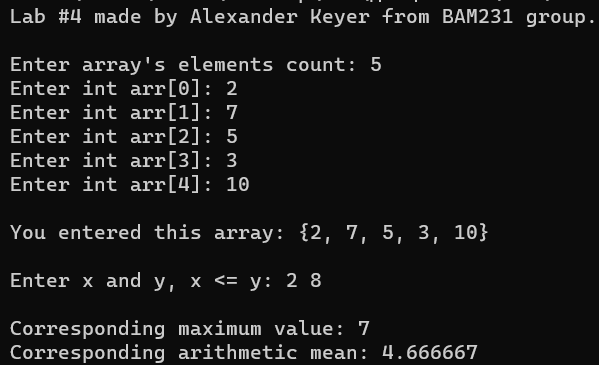
\includegraphics[width=400px]{test_1}
	Программа сработала корректно.
	
	\subsection*{Тест № 2}
	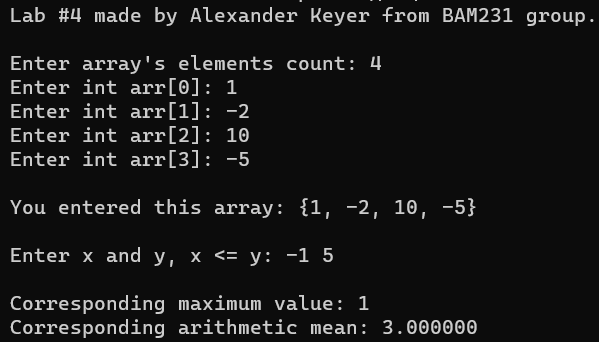
\includegraphics[width=400px]{test_2}
	Программа сработала корректно.
	
	\subsection*{Тест № 3}
	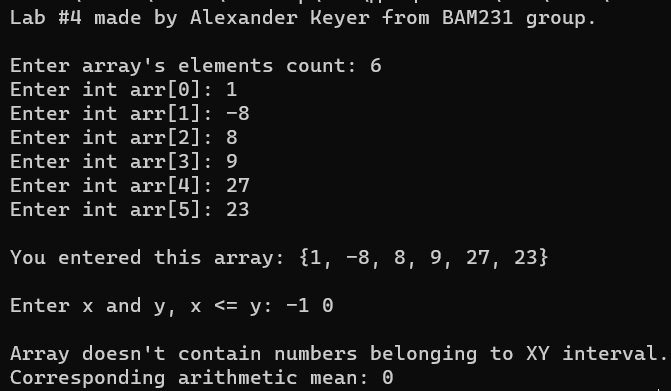
\includegraphics[width=400px]{test_3}
	Программа сработала корректно.
	
	\subsection*{Тест № 4}
	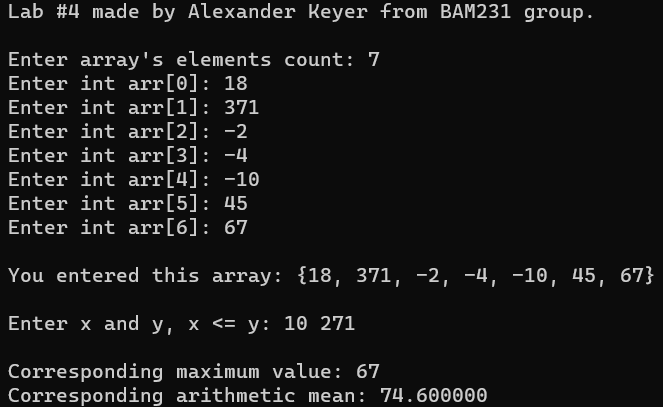
\includegraphics[width=400pt]{test_4}
	Программа сработала корректно.
	
\end{document}
